% 第二部分从 08:00 讲到 19:00，共 660 秒。
\newcommand{\studyline}[2]{\par\noindent\accenttext{#1}\hspace{.7em}#2\par}
\section{数据与基线}

\begin{frame}[t,label=group-start]{第二部分　用 CIFAR-100 检验 TANL 的改进}
    \pdfbookmark[3]{08:00　数据与评测设置}{timing-480}
    \small
    \studyline{测试任务}{模型认识 CIFAR-100 的 100 类。每次取它的 10,000 张测试图作分布内样本（ID），与下列一组分布外图像（OOD）打乱，逐批检测。}
    \vspace{2mm}
    \begin{tabular*}{\linewidth}{@{\extracolsep{\fill}}cccc@{}}
        
\includegraphics[height=1.18cm]{cifar10-airplane.png} &
        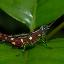
\includegraphics[height=1.18cm]{tiny-imagenet-insect.jpg} &
        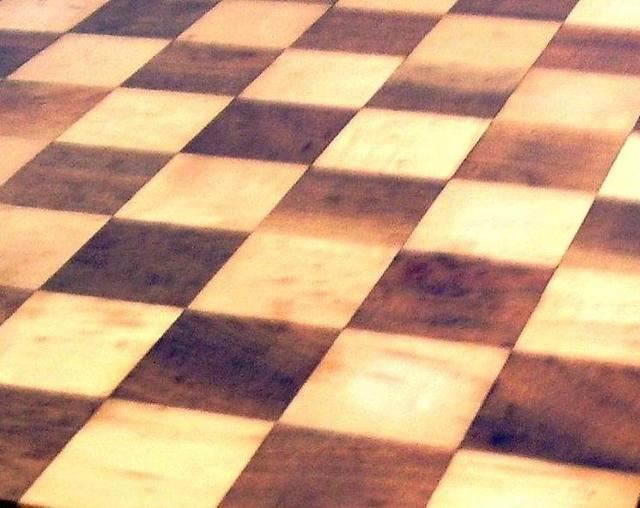
\includegraphics[height=1.18cm,width=2.3cm,keepaspectratio]{dtd-chequered.jpg} &
        
\includegraphics[height=1.18cm]{svhn-digit.jpg}\\
        CIFAR-10 & Tiny ImageNet & DTD 纹理 & SVHN 街景数字\\
        近分布，10,000 张 & 近分布，6,526 张 & 远分布，5,640 张 & 远分布，26,032 张
    \end{tabular*}
    \vspace{2.6mm}
    \studyline{共同参数}{冻结 CLIP ViT-B/16，每批 200 张。从 69,929 个候选词中每批选 1,000 个负词，正负队列各最多保留 300 个特征，历史激活权重为 0.95。}
    \vspace{1.7mm}
    \studyline{如何读结果}{种子 0、1、2 改变图像顺序，每次重建队列。检测表取三次均值。FPR95 是检出 95\% OOD 时误拒的 ID 比例，越低越好。AUROC 越高越好。}
    \note{65 秒。以第一列为例，一条测试流含一万张 CIFAR-100 和一万张 CIFAR-10，共两万张。后面几页凡是说 CIFAR-10 的检测结果，都指这对数据。Tiny ImageNet、DTD 和 SVHN 各自与同一万张 ID 配对，四种 OOD 分开评测。模型在流中看不到真实身份，真实标签只用于事后评价。三个种子对应相同图像的三种顺序。
    \par 数据与参数见 \datafile{protocol.yml}、\datafile{multimodal/README.md} 和 \datafile{multimodal/seeds.csv}。四张示例图来自各自的测试清单。}
\end{frame}

\begin{frame}[t]{基线校准　提示句式能解释多少复现差距？}
    \pdfbookmark[3]{09:05　论文数值、公开代码与统一提示}{timing-545}
    \small
    \studyline{论文与公开代码}{论文给出 \mbox{\texttt{The nice <label>}}。公开代码用 \mbox{\texttt{The nice \{\}.}} 编码已知类和名词，用 \mbox{\texttt{This is a \{\} photo.}} 编码形容词。花括号里填入标签词。}
    \vspace{1.4mm}
    \studyline{改动与设置}{仅把 11,453 个形容词改用名词句式。10,000 张 CIFAR-100（ID）与 10,000 张 CIFAR-10（OOD）混成 20,000 张。固定原队列、原图和全类评分。}
    \vspace{2mm}
    \begin{tabular*}{\linewidth}{@{\extracolsep{\fill}}lrrr@{}}
        \toprule
        CIFAR-10 作 OOD & FPR95 $\downarrow$（\%） & AUROC $\uparrow$（\%） & 正队列入队数（种子 0）\\ \midrule
        论文表 A10(b) & 56.32 & 80.47 & 未报告\\
        本地公开实现 & 72.32 & 72.94 & 19 张\\
        本地统一提示 & 63.80 & 82.24 & 309 张\\ \bottomrule
    \end{tabular*}
    \vspace{2mm}
    \studyline{结果}{统一句式使本地 FPR95 降低 8.52 个百分点，仍高于论文值。19 张是整条混合流里累计入队的图，事后核对均来自 CIFAR-100。}
    \note{75 秒。论文表 A10(b) 是作者报告值。中间一行是我们把公开实现放在本地跑出的结果，作者的 CIFAR 脚本引用了一份缺失的配置。在种子零，换回上游原始后处理得到的两万个分数与本地逐个相同。表中最后两行只改变形容词模板，保留句点，图像、词库和超参数都相同。最后一列统计两万张测试图里累计有多少张被当作高置信 ID 接纳，与队列同时最多保存三百个特征是不同的量。接下来的方法对照用本地统一提示起步。
    \par \paperref{7}{原论文第 4.1 节}，\paperref{16}{表 A10(b)}。本地记录见 \datafile{metrics.csv}、\datafile{upstream_check.json}、\datafile{diagnostics/summary.csv} 及 \datafile{improvements/cifar10_seeds.csv}。}
\end{frame}

\section{检测方法}

\begin{frame}[t]{实验一　让更多真实 ID 进入正队列，误报会减少吗？}
    \pdfbookmark[3]{10:20　正队列的入队门槛}{timing-620}
    \small
    \studyline{原论文的入队规则}{模型先用已有分数估计 ID 与 OOD 的分界，再用置信间隔参数 $g=0.2$ 提高正队列门槛。分数超过门槛的图像才入队，供后续选词。}
    \vspace{1mm}
    \studyline{我们的改动}{初步 ID 分数超过最近至多 1,000 张测试图分数的第 80 百分位就进正队列。首批用本批估计。剩余图像沿用原负队列门槛。}
    \vspace{1mm}
    \studyline{实验设置}{固定统一提示、原图、全类评分。每组用 10,000 张 CIFAR-100 作 ID，分别混入下表三种 OOD。}
    \vspace{1.5mm}
    \begin{tabular*}{\linewidth}{@{\extracolsep{\fill}}llrrr@{}}
        \toprule
        & CIFAR-10 流，种子 0 & \multicolumn{3}{c}{FPR95（\%，三种顺序均值）$\downarrow$}\\
        \cmidrule(lr){3-5}
        正队列门槛 & 真实 ID 数 / 入队总数 & CIFAR-10 & Tiny ImageNet & DTD\\ \midrule
        原门槛 & 303 / 309 & 63.80 & 72.02 & 21.48\\
        新门槛 & \textbf{3,586} / 4,071 & 63.88 & \textbf{66.83} & \textbf{17.93}\\ \bottomrule
    \end{tabular*}
    \vspace{1.6mm}
    \studyline{结果}{入队图像中真实 ID 的占比从 98.1\% 降至 88.1\%。Tiny ImageNet 和 DTD 的误报率下降，CIFAR-10 基本持平。}
    \note{105 秒。同样使用统一提示，原门槛收到三百零三个真实 ID，新门槛收到三千五百八十六个，约为原来的十二倍。代价是也混进了更多 OOD。原论文的正门槛为 $\gamma+(1-\gamma)g$，其中 $\gamma$ 由历史分数估计。本地新规则在第二批起只看此前真实图像的分数，历史不足一千时使用已有部分。已进正队列的图从负侧剔除。Tiny ImageNet 降低 5.19 个百分点，DTD 降低 3.55 个百分点。DTD 是确定入队规则后首次使用的验证集。CIFAR-10 的 FPR95 增加 0.08 个百分点，AUROC 从 82.24\% 升至 82.77\%。
    \par \paperref{4}{TANL 如何设置正、负队列的入队门槛}。\datafile{improvements/quantile.yml}、\datafile{improvements/positive.yml} 及 \datafile{improvements/README.md} 收录了配置、计数和逐种子对照。}
\end{frame}

\begin{frame}[t,label=negative-reranking]{实验二　把对图像反应相似的负词后移，能减少误报吗？}
    \pdfbookmark[3]{12:05　按图像响应重排负标签}{timing-725}
    \small
    \studyline{原论文的排序}{TANL 按激活差选前 1,000 个负词，排名越靠前，参与评分的次数越多。例如，若“货船”和“轮船”总在相同的照片上得高分，就可能重复强调同一线索。}
    \vspace{1mm}
    \studyline{我们的改动}{先取激活差最高的 2,000 个词，比较它们在本批图像上的响应。若一个词与任一更靠前的词的相关系数达到 0.90，就把它后移，再取前 1,000 个词评分。}
    \vspace{1mm}
    \studyline{实验设置}{ID 均为 10,000 张 CIFAR-100。OOD 取 CIFAR-10（10,000 张）或 \mbox{Tiny ImageNet}（6,526 张）。固定统一提示、原论文的入队规则和全类评分。每批 200 张，取三种顺序的均值。}
    \vspace{1.5mm}
    \begin{tabular*}{\linewidth}{@{\extracolsep{\fill}}lrrrrr@{}}
        \toprule
        & & \multicolumn{2}{c}{FPR95（\%）$\downarrow$} & \multicolumn{2}{c}{AUROC（\%）$\uparrow$}\\
        \cmidrule(lr){3-4}\cmidrule(l){5-6}
        OOD 数据集 & 每批平均换入词数 & 原排序 & 重排 & 原排序 & 重排\\ \midrule
        CIFAR-10 & 197 & 63.80 & \textbf{64.72} & 82.24 & 81.80\\
        Tiny ImageNet & 221 & 72.02 & \textbf{71.80} & 76.74 & 76.82\\ \bottomrule
    \end{tabular*}
    \vspace{1.4mm}
    \studyline{结果}{每批换掉约五分之一的负词。CIFAR-10 的误报增加，\mbox{Tiny ImageNet} 的误报略降。}
    \note{105 秒。“货船”和“轮船”是假设的例子。判定时看两个词在同一批图像上是否一起得高分、一起得低分。对每个词，收集它在本批各图像上的激活值，按皮尔逊相关系数与排在它前面的词比较。把达到门槛的词放到其余候选词之后，两组词各自保留原来的顺序，最后选一千个。这里改的是用来评分的负标签排名，正负队列仍按原规则存图像特征。换入词数统计重排后的前一千个词里，有多少原先排在一千名以外，表中四舍五入到整数。CIFAR-10 的三种顺序误报都增加，Tiny ImageNet 的三种顺序里有两次改善、一次退步。
    \par \paperref{5}{TANL 的负词排序与图像评分}。参数和换入词数见 \datafile{improvements/ablation.py}。逐次结果见 \datafile{improvements/cifar10_seeds.csv}、\datafile{improvements/tin_seeds.csv}。}
\end{frame}

\begin{frame}[t]{实验三　图像必须明显匹配某个已知类，检测会更准吗？}
    \pdfbookmark[3]{13:50　全类评分与 Top-1 联合评分}{timing-830}
    \small
    \studyline{实验设置}{10,000 张 CIFAR-100 分别配表中四种 OOD。固定统一提示、原图和第 80 百分位正队列门槛。两种评分共用入队样本、负词排名和三种测试顺序。}
    \vspace{3mm}
    \begin{columns}[T,onlytextwidth]
        \begin{column}{.48\linewidth}
            \lead{原论文的全类评分}
            按排名逐个加入负词，每次把 100 个已知类的概率相加。对这些概率和取平均，得到图像的 ID 分数 $S$。
            \par\vspace{2.2mm}
            \lead{我们的改动}
            在 100 个已知类内部求概率，取最大值 $p_{\max}$。新的 Top-1 联合分数为 $S\,p_{\max}$。多个类得分相近时，乘子就小。
        \end{column}
        \begin{column}{.47\linewidth}
            \lead{检测结果}
            \vspace{1.2mm}
            \begin{tabular*}{\linewidth}{@{\extracolsep{\fill}}lrr@{}}
                \toprule
                FPR95（\%）$\downarrow$ & 全类 & Top-1 联合\\ \midrule
                CIFAR-10 & 63.88 & \textbf{54.06}\\
                Tiny ImageNet & 66.83 & 65.90\\
                DTD 纹理 & 17.93 & \textbf{33.20}\\
                SVHN 街景数字 & 1.53 & 1.20\\ \bottomrule
            \end{tabular*}
        \end{column}
    \end{columns}
    \vspace{2.7mm}
    \studyline{结果}{CIFAR-10 的 FPR95 降低 9.82 个百分点，同一改动却让 DTD 增加 15.27 个百分点。}
    \note{85 秒。全类评分允许多个已知类别分别贡献少量概率。我们的设想是，若已知图像通常明确指向其中一类，可以把这一信息用于拒识。这里的最大概率是只在一百个已知类上做 softmax 的结果。用同一批输入、队列与负词排序，只替换最终评分。CIFAR-10 的大幅改善和 DTD 的明显退步同时存在，Tiny ImageNet、SVHN 的变化则较小。
    \par \paperref{5}{TANL 如何汇总已知类概率来计算图像分数}。表格取自 \datafile{multimodal/summary.csv} 中统一提示和原图的 \datafile{all}、\datafile{joint1} 两组。}
\end{frame}

\begin{frame}[t]{实验四　加入同一张图的水平翻转，能减少误报吗？}
    \pdfbookmark[3]{15:15　原图与水平翻转双视角}{timing-915}
    \small
    \studyline{实验设置}{10,000 张 CIFAR-100 分别配表中四种 OOD。固定统一提示、第 80 百分位正队列门槛和全类评分。两种视角配置各自按三种顺序重跑队列。}
    \vspace{2.4mm}
    \begin{columns}[T,onlytextwidth]
        \begin{column}{.47\linewidth}
            \lead{从单视角到双视角}
            \vspace{.8mm}
            \begin{tabular}{@{}c@{\hspace{3mm}}c@{}}
                
\includegraphics[height=1.4cm]{cifar10-airplane.png} &
                \reflectbox{
\includegraphics[height=1.4cm]{cifar10-airplane.png}}\\
                原图 & 水平翻转
            \end{tabular}
            \par\vspace{1mm}
            原 TANL 只编码原图。我们分别编码两个视角，将单位向量等权平均后再归一化。
        \end{column}
        \begin{column}{.47\linewidth}
            \lead{检测结果}
            \vspace{1.2mm}
            \begin{tabular*}{\linewidth}{@{\extracolsep{\fill}}lrr@{}}
                \toprule
                FPR95（\%）$\downarrow$ & 单视角 & 双视角\\ \midrule
                CIFAR-10 & 63.88 & 63.19\\
                Tiny ImageNet & 66.83 & 66.51\\
                DTD 纹理 & 17.93 & 16.98\\
                SVHN 街景数字 & 1.53 & 1.48\\ \bottomrule
            \end{tabular*}
        \end{column}
    \end{columns}
    \vspace{2mm}
    \studyline{收益与代价}{四组 FPR95 均降低，降幅为 0.05 至 0.96 个百分点。ID 分类准确率从 63.21\% 升至 63.98\%，每张图多做一次视觉编码。}
    \note{75 秒。左侧是同一架飞机，第二张来自对第一张做水平翻转。两个特征都归一化，等权平均后再归一化，所得向量用于入队、选词和最终打分。这次两列都用全类评分，可以单独看双视角的作用。CIFAR-100 分类准确率也从 63.21\% 升至 63.98\%。SVHN 的 FPR95 略降，而 AUROC 从 99.64\% 略降至 99.63\%。降幅按未四舍五入的均值计算。
    \par \datafile{multimodal/dual_view.yml}、\datafile{multimodal/summary.csv}、\datafile{multimodal/dual_view_raw_checks.csv}。照片来自 CIFAR-10 测试集。}
\end{frame}

\section{验证与结论}

\begin{frame}[t]{实验五　在三个数据集上选出的配置，能推广到街景数字吗？}
    \pdfbookmark[3]{16:30　配置选择与预留数据集}{timing-990}
    \small
    \studyline{原论文与改动}{论文表 A10(b) 逐集报告 TANL。我们额外考察跨数据集选型。固定第 80 百分位正队列门槛，比较 6 种图文表示和 5 种评分，共 30 个配置。}
    \vspace{1.4mm}
    \studyline{实验设置}{每组均有 10,000 张 CIFAR-100 作 ID。对 CIFAR-10、Tiny ImageNet 和 DTD 的 FPR95 取等权平均，选最低者，再用 SVHN 的 26,032 张 OOD 图检验。}
    \vspace{2mm}
    \begin{tabular*}{\linewidth}{@{\extracolsep{\fill}}lrr@{}}
        \toprule
        FPR95（\%，越低越好） & 选型用的三组均值 & 预留 SVHN\\ \midrule
        单模板、原图、全类评分（对照） & 49.55 & 1.53\\
        双模板、双视角、全类评分（入选） & \textbf{48.38} & \textbf{2.10}\\ \bottomrule
    \end{tabular*}
    \vspace{2mm}
    \studyline{入选配置}{将每个标签分别填入 \mbox{\texttt{The nice \{\}.}} 和 \mbox{\texttt{\{\}.}} 两种模板，等权融合文本特征。图像用原图和水平翻转，评分保留全部 100 个已知类。}
    \vspace{1.2mm}
    \studyline{结果}{选型三组的平均误报率下降，预留 SVHN 上的三种顺序却都退步。}
    \note{90 秒。所有配置使用统一的分位数正队列。六种表示依次为原模板原图、原模板翻转图、原模板双视角、词名模板原图、双模板原图、双模板双视角。五种评分为全类、Top-1 和 Top-3 联合、Top-1 和 Top-3 竞争。ID 与候选负词都按同样的模板编码。三组数据各占三分之一权重，各组 FPR95 先对三个种子求均值。对照是统一单模板、原图和全类评分。胜出组合对预留集的 AUROC 也从 99.64\% 降到 99.47\%。这说明按前三组挑出的配置在这个新来源上没有延续收益。
    \par \paperref{16}{原论文表 A10(b)}。\datafile{multimodal/selected.yml}、\datafile{multimodal/seeds.csv}、\datafile{multimodal/selected_raw_checks.csv}。}
\end{frame}

\begin{frame}[t]{回到论文表 A10(b)　每一步对 CIFAR-10 的贡献}
    \pdfbookmark[3]{18:00　组合结果与论文对照}{timing-1080}
    \small
    \studyline{对照条件}{同一批 CIFAR-100 ID 和 CIFAR-10 OOD 各 10,000 张。本地各行都用原始负词排序、全类评分和相同的三种顺序，依次加入一项改动。}
    \vspace{2.5mm}
    \begin{tabular*}{\linewidth}{@{\extracolsep{\fill}}lrr@{}}
        \toprule
        方法 & FPR95 $\downarrow$（\%） & AUROC $\uparrow$（\%）\\ \midrule
        论文报告的 TANL & 56.32 & 80.47\\ \midrule
        本地公开实现 & 72.32 & 72.94\\
        \quad 统一形容词与名词的提示 & 63.80 & 82.24\\
        \quad 再改正队列门槛 & 63.88 & 82.77\\
        \quad 再加水平翻转双视角 & \textbf{63.19} & \textbf{82.93}\\ \bottomrule
    \end{tabular*}
    \vspace{2.3mm}
    \studyline{逐项对照}{双视角组合的 FPR95 比本地公开实现低 \textbf{9.13 个百分点}，其中统一提示贡献最大。}
    \vspace{1.2mm}
    \studyline{事后按 CIFAR-10 选型}{双模板、双视角、Top-1 联合取得 FPR95 53.14\%、AUROC 84.24\%，两项都优于论文报告值。同一配置在 DTD 上的 FPR95 升至 34.44\%。}
    \note{60 秒。最后一行是单模板、双视角和全类评分的组合，和预留集选出的双模板配置要分开理解。本地 FPR95 降低 9.13 个百分点，AUROC 从 72.94\% 升至 82.93\%。若只看 CIFAR-10，Top-1 联合评分还能压低 FPR95，但纹理误报大幅上升。正队列在 Tiny ImageNet 和 DTD 上的收益比在 CIFAR-10 上更明显。19 分钟结束，留 1 分钟机动。
    \par \paperref{16}{原论文表 A10(b)}。\datafile{metrics.csv}、\datafile{diagnostics/summary.csv}、\datafile{improvements/cifar10_sides_summary.csv}、\datafile{multimodal/summary.csv} 与 \datafile{multimodal/a10_joint1.yml}。}
\end{frame}
